\section{Methodology & Process}
% zimmerman and Forlizzi (2004), knowledge opportunity map in the design process

\section{Analysis}

\begin{figure}[H]
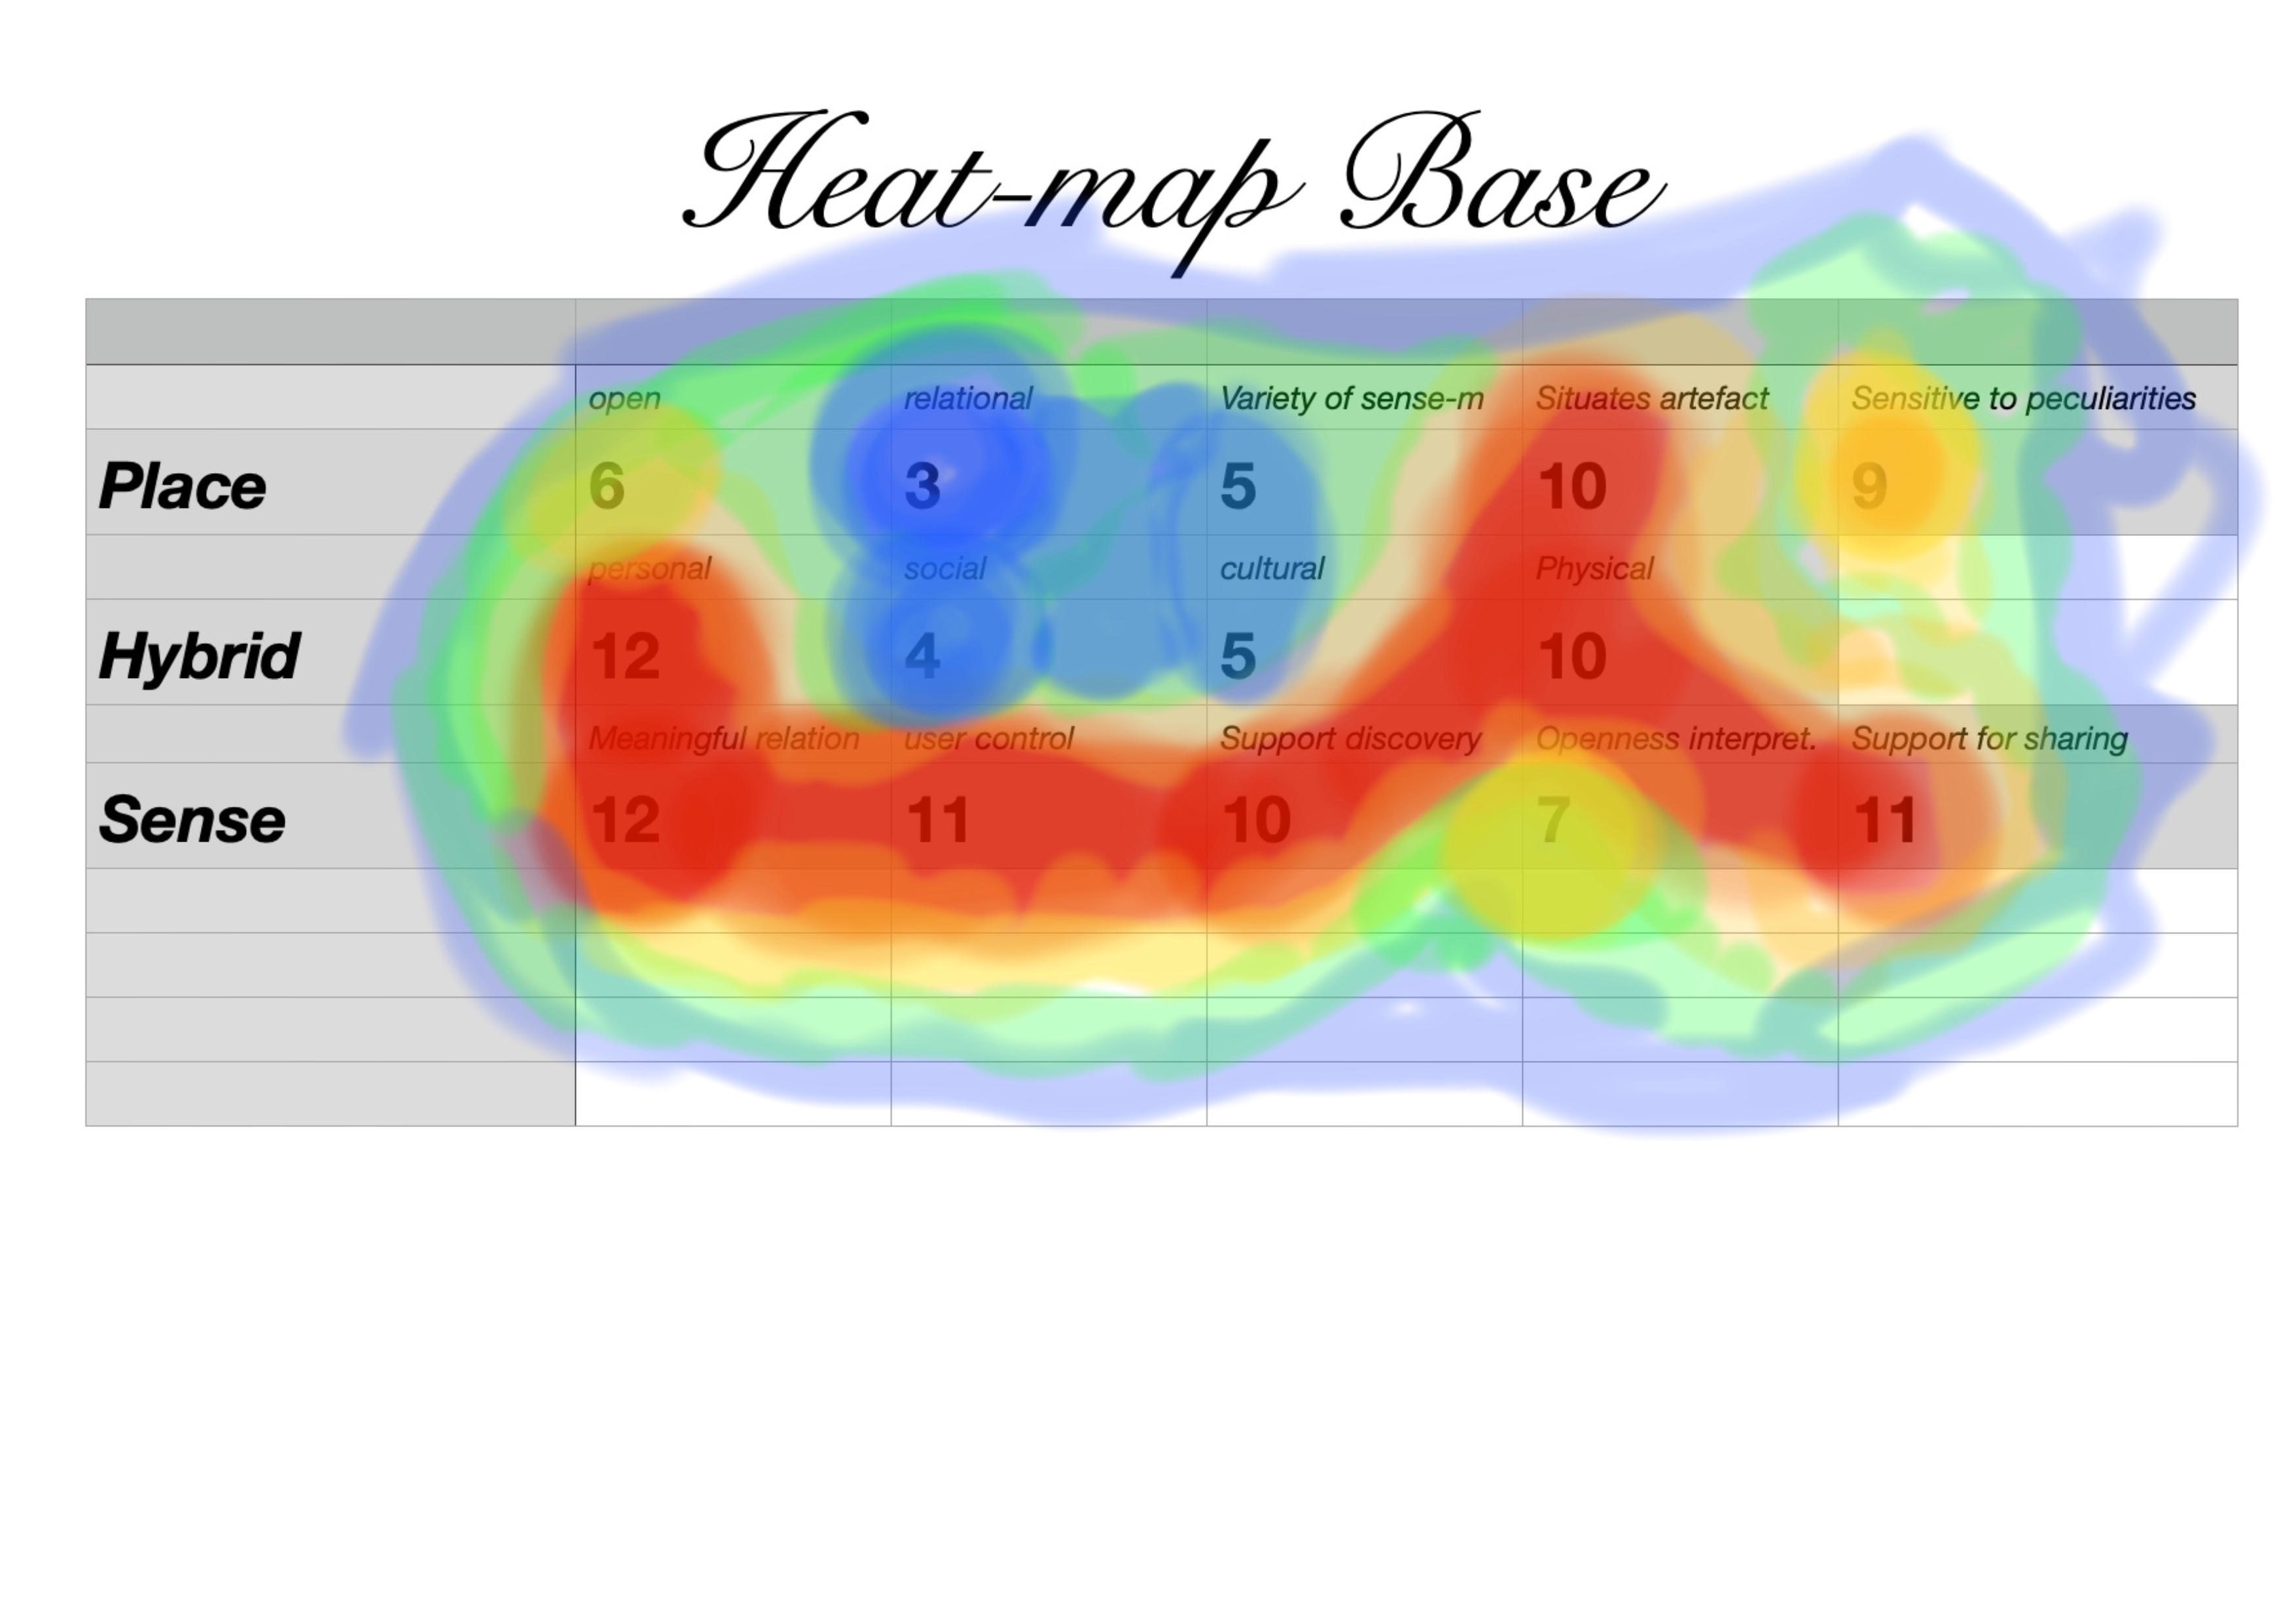
\includegraphics[width=12.5cm]{pictures/dataset/heatmap.jpg}
\caption{Heatmap version 1, Munch shadows is weighted as one}
\end{figure}

\section{Datagathering: observation guide}
\begin{figure}[H]
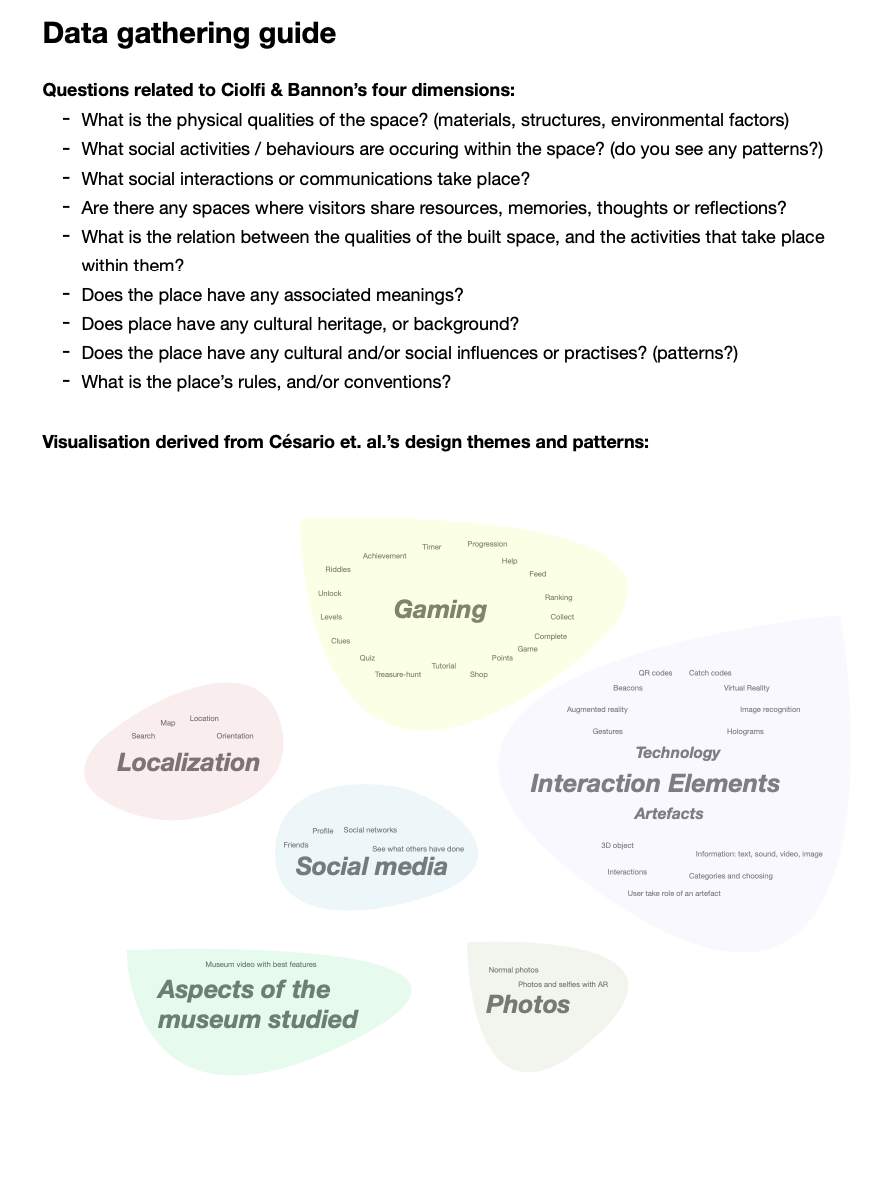
\includegraphics[width=13cm]{pictures/appendix/datagathering.png}
\centering 
\end{figure}

\section{Datagathering: interview guide}
\section{Dataset: Interactive Installations}

\begin{figure}[H]
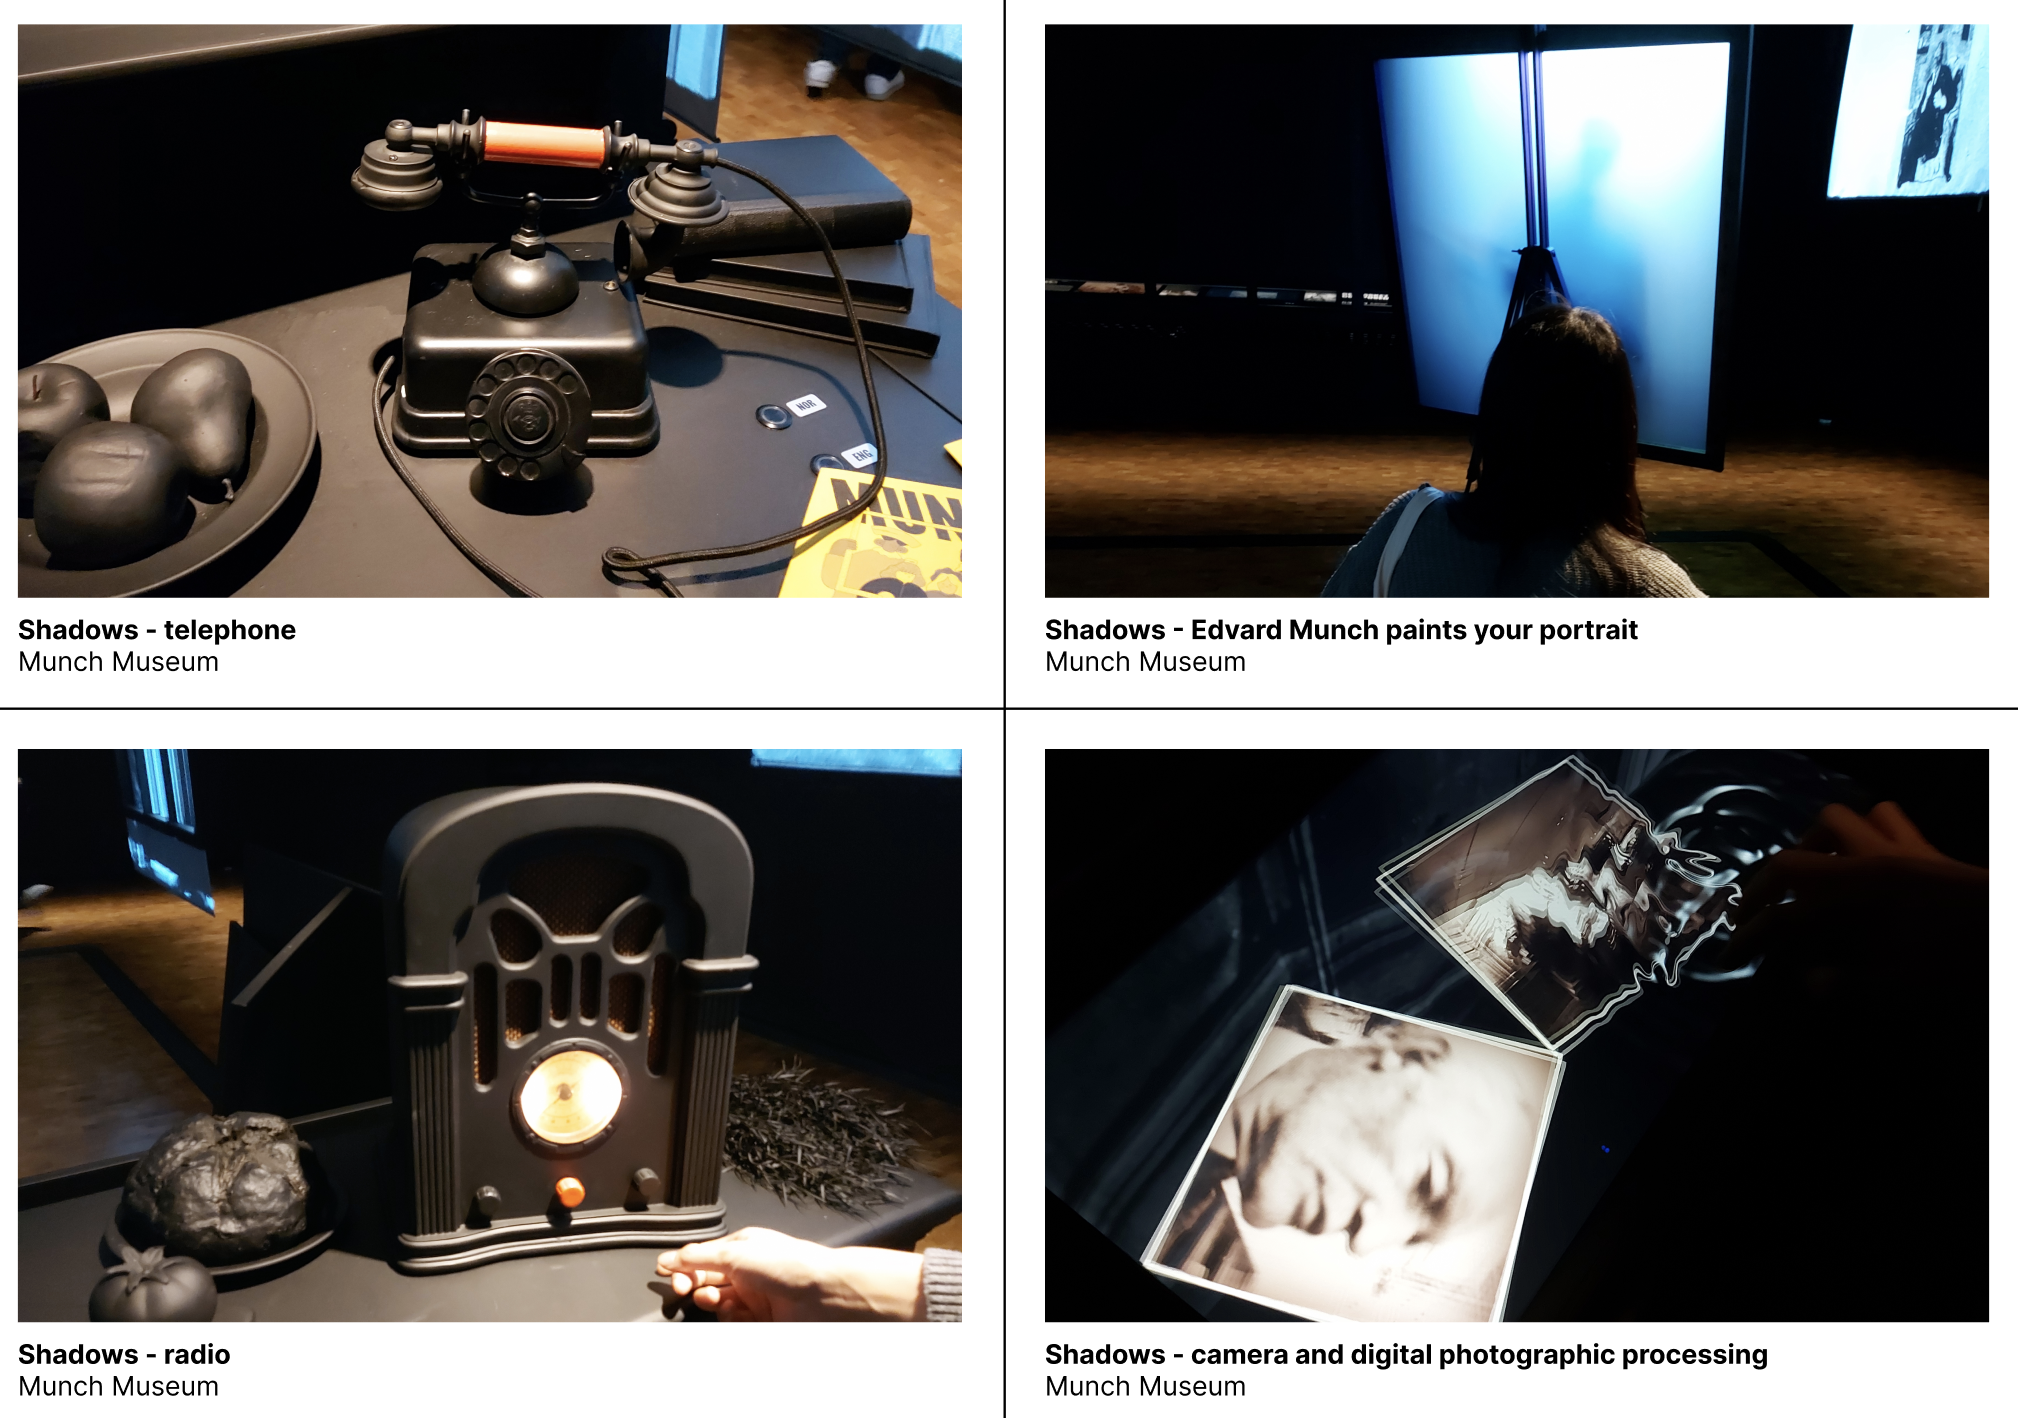
\includegraphics[width=13cm]{pictures/dataset/munch_1.png}
\centering 
\end{figure}

\begin{figure}[H]
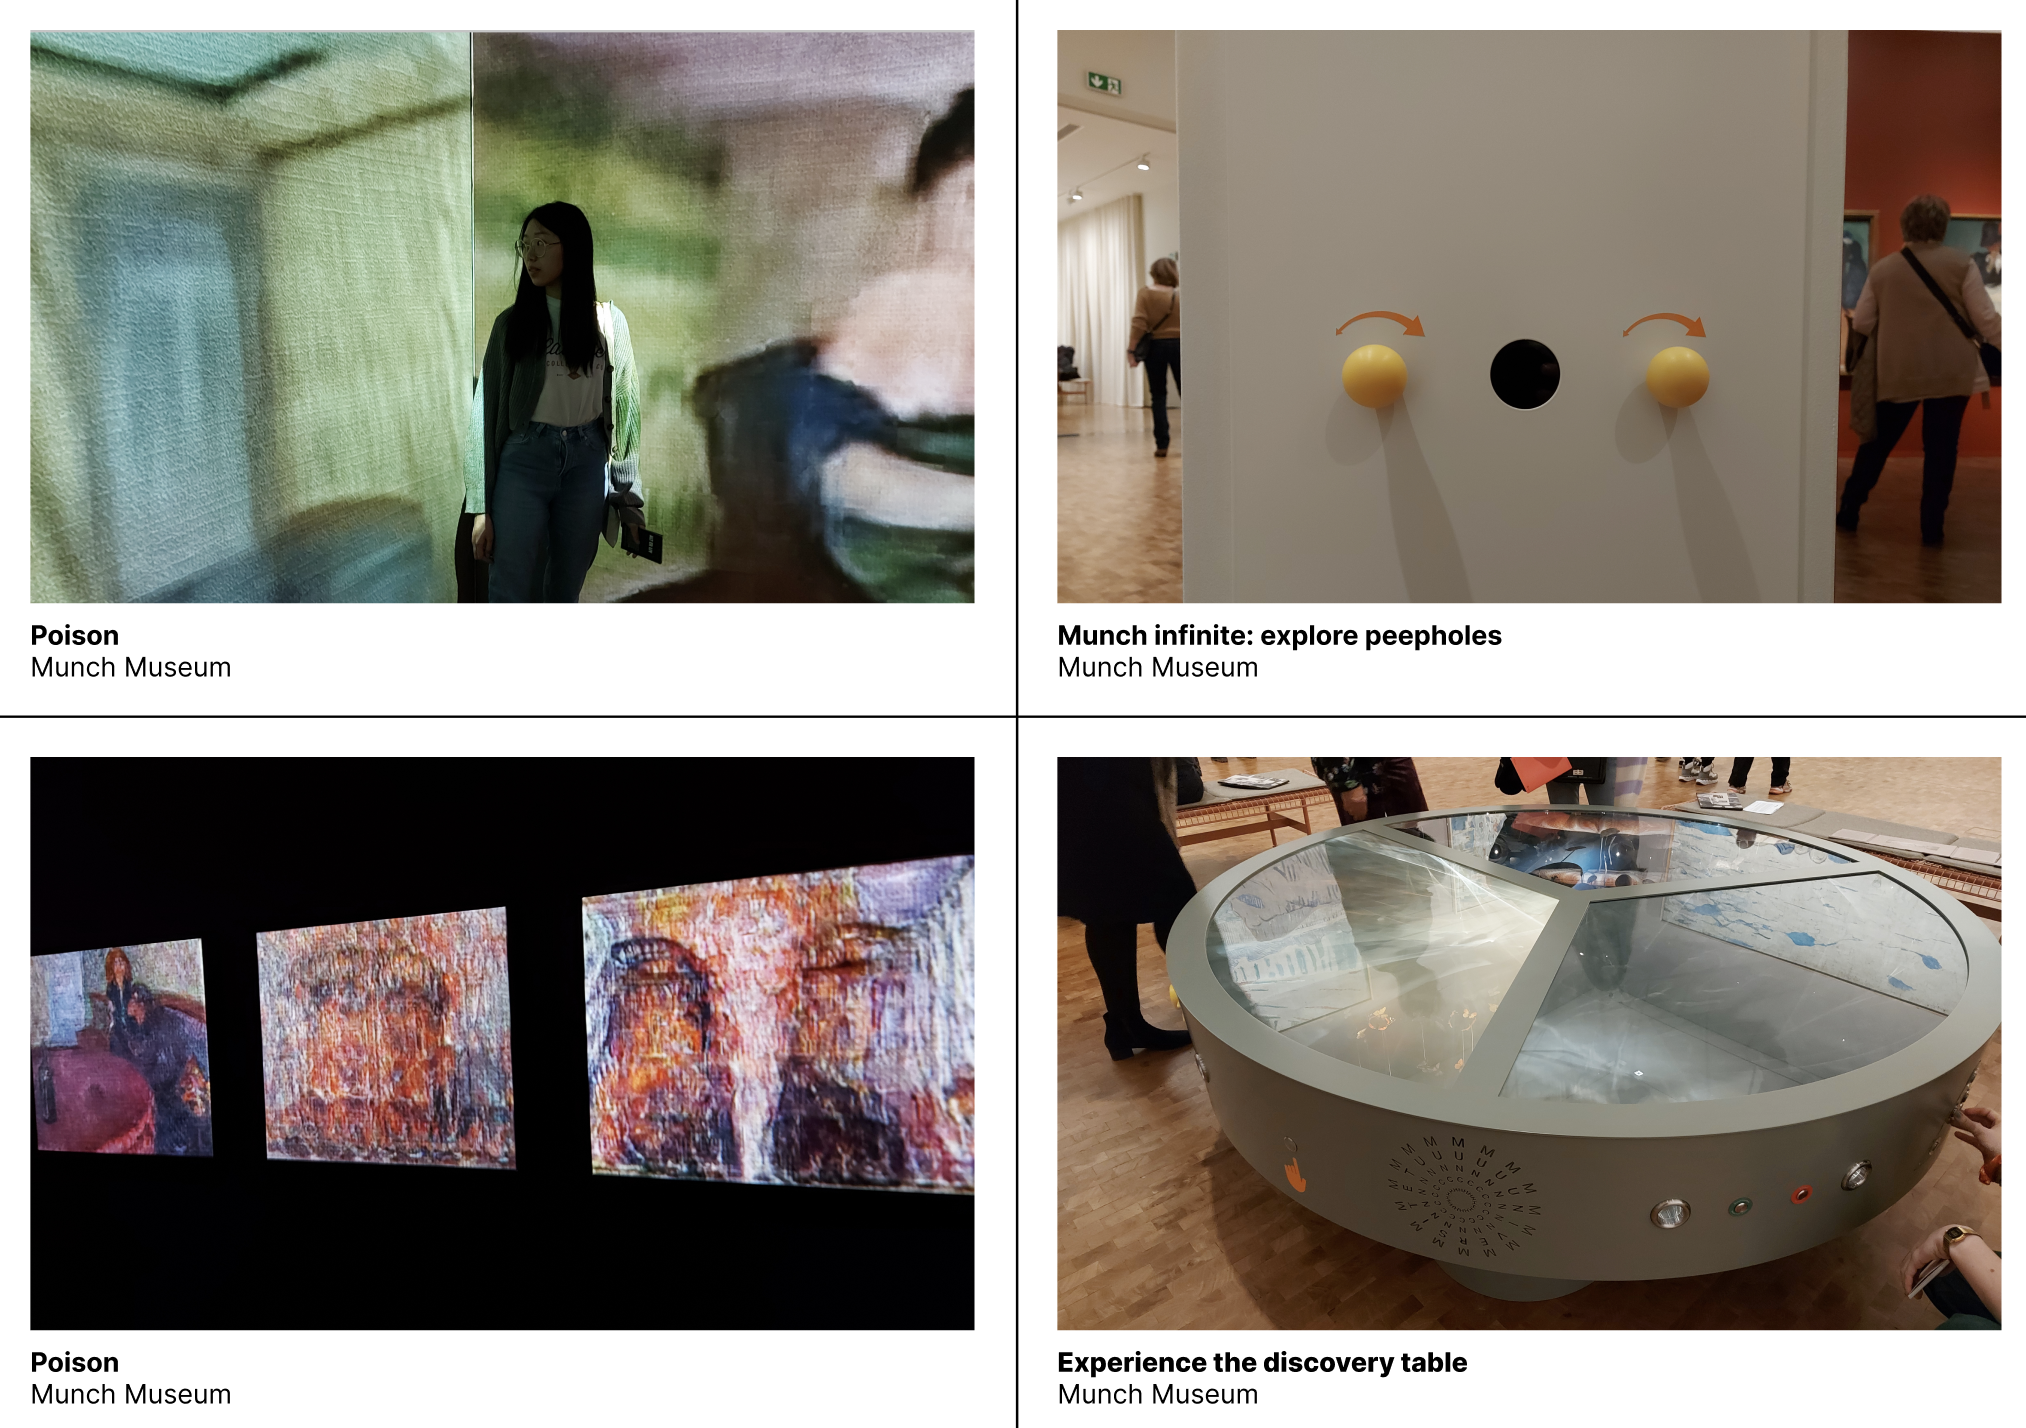
\includegraphics[width=13cm]{pictures/dataset/munch_2.png}
\centering 
\end{figure}

\begin{figure}[H]
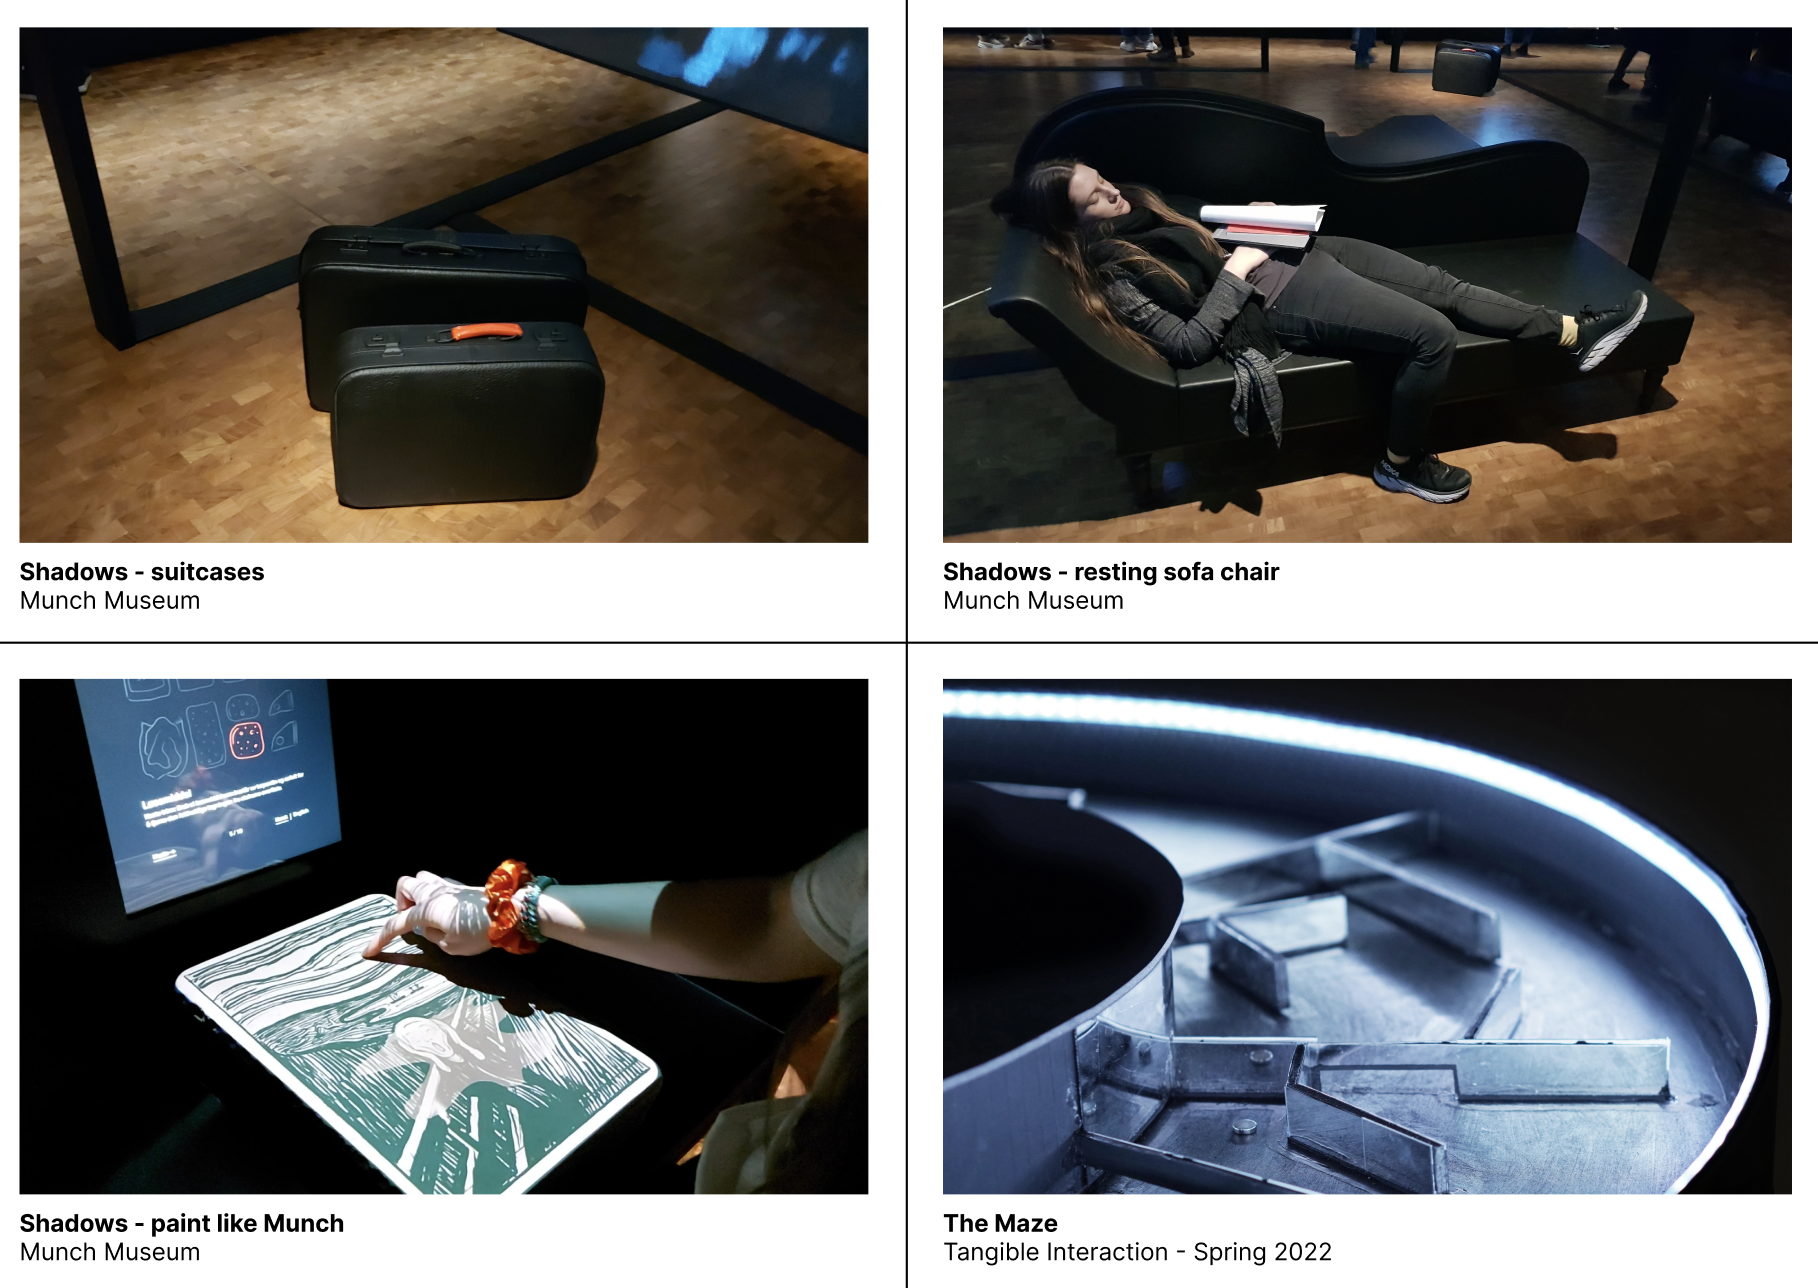
\includegraphics[width=13cm]{pictures/dataset/munch_3.png}
\centering 
\end{figure}

\begin{figure}[H]
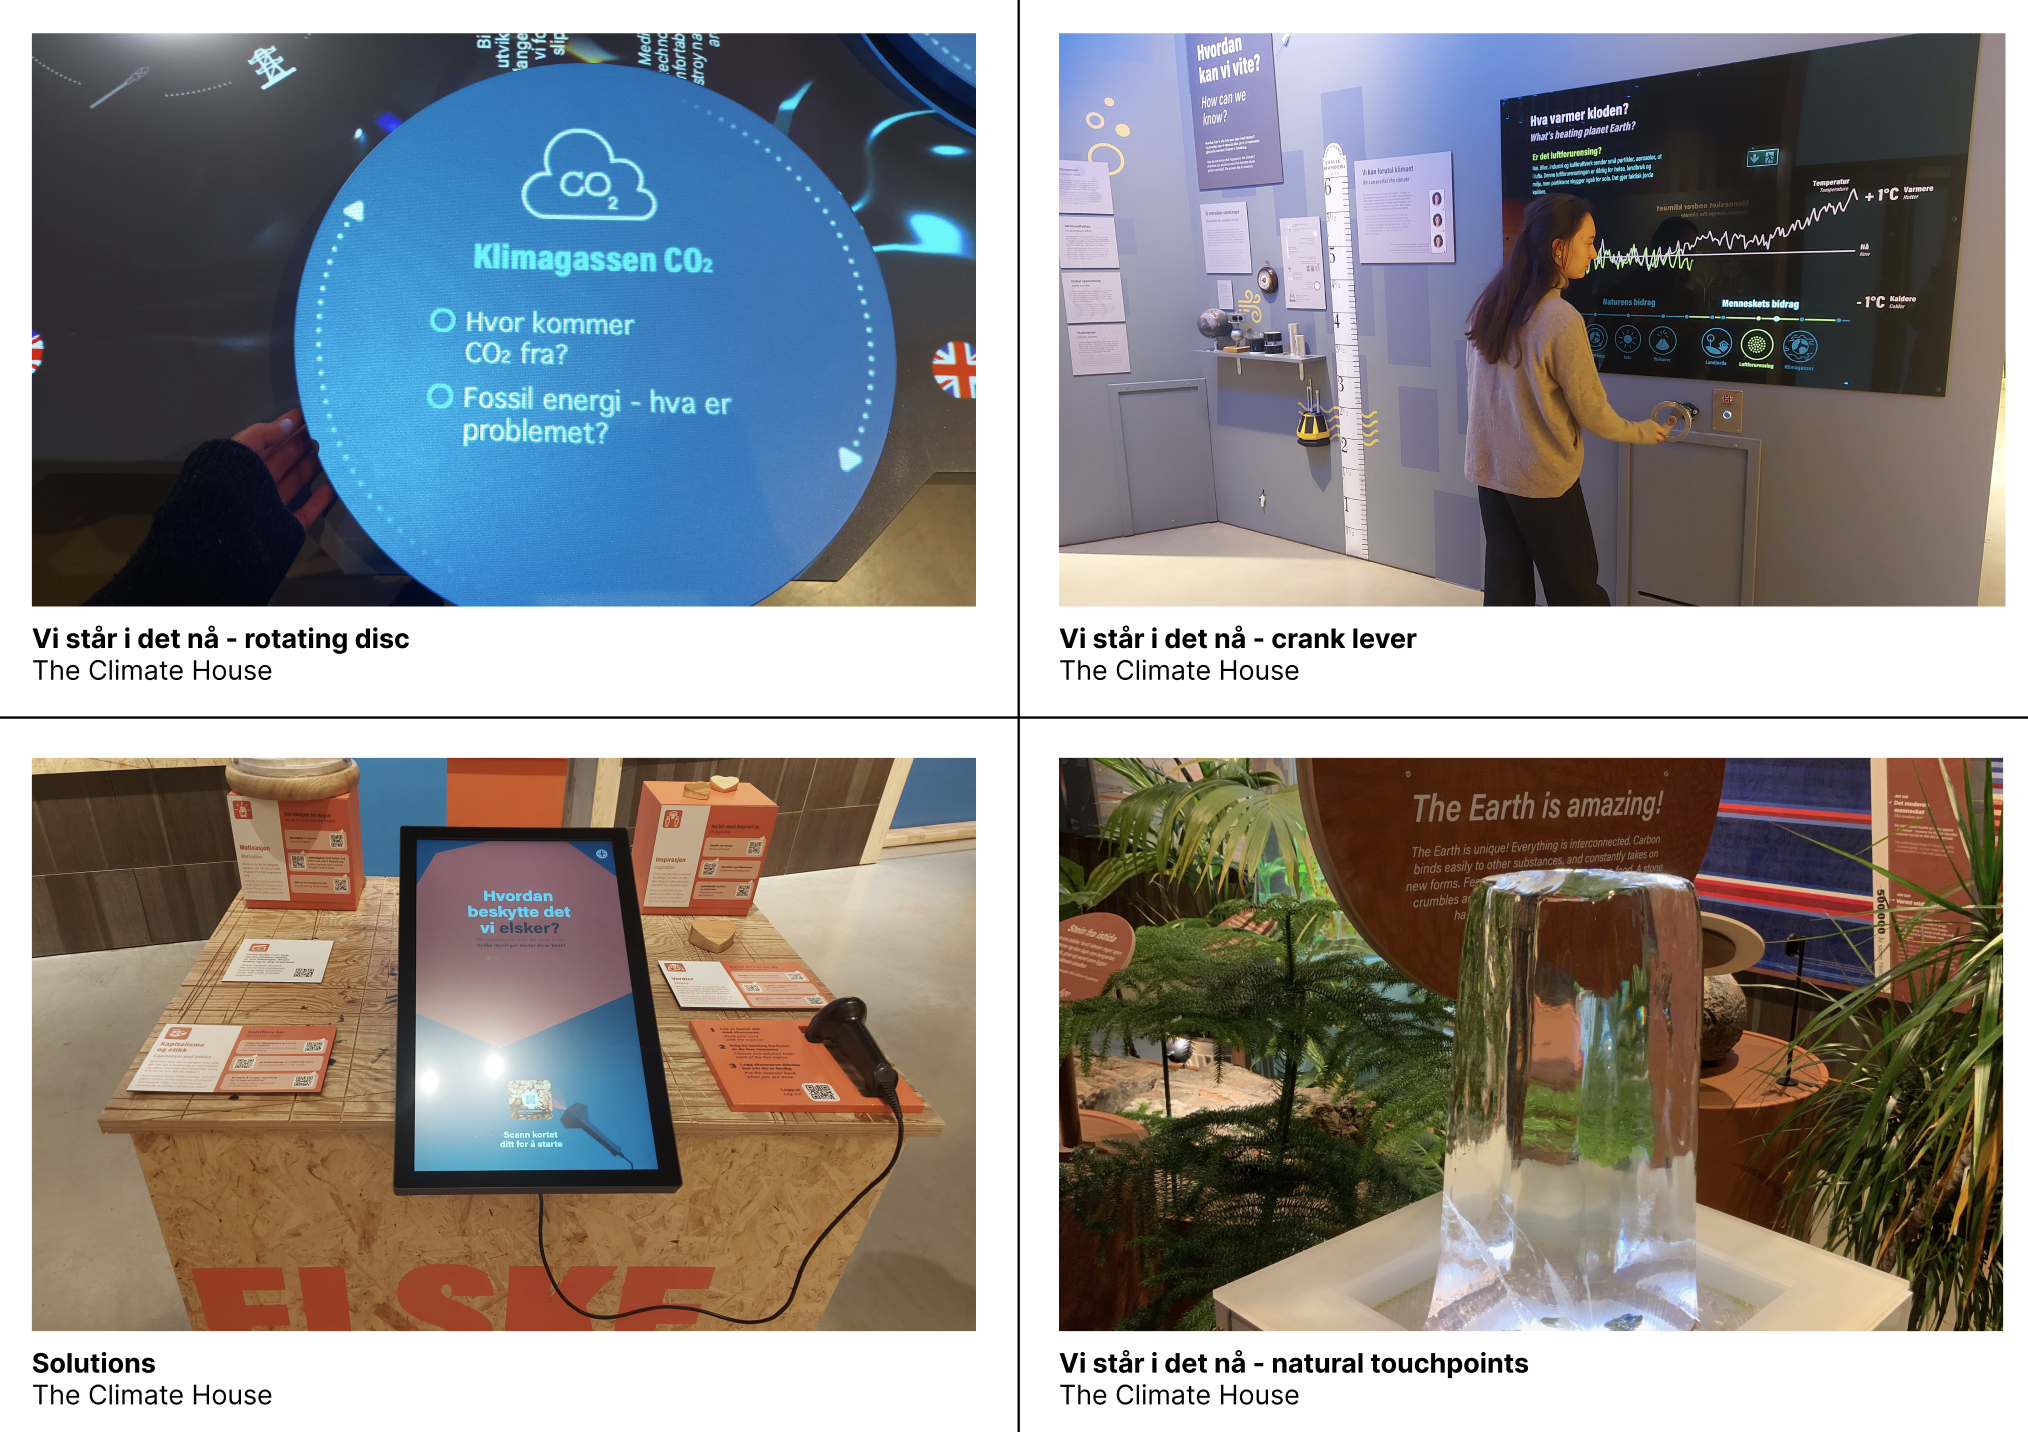
\includegraphics[width=13cm]{pictures/dataset/klimahuset.png}
\centering 
\end{figure}

\begin{figure}[H]
\includegraphics[width=13cm]{pictures/dataset/Qi.pdf}
\centering 
\end{figure}


\begin{figure}[H]
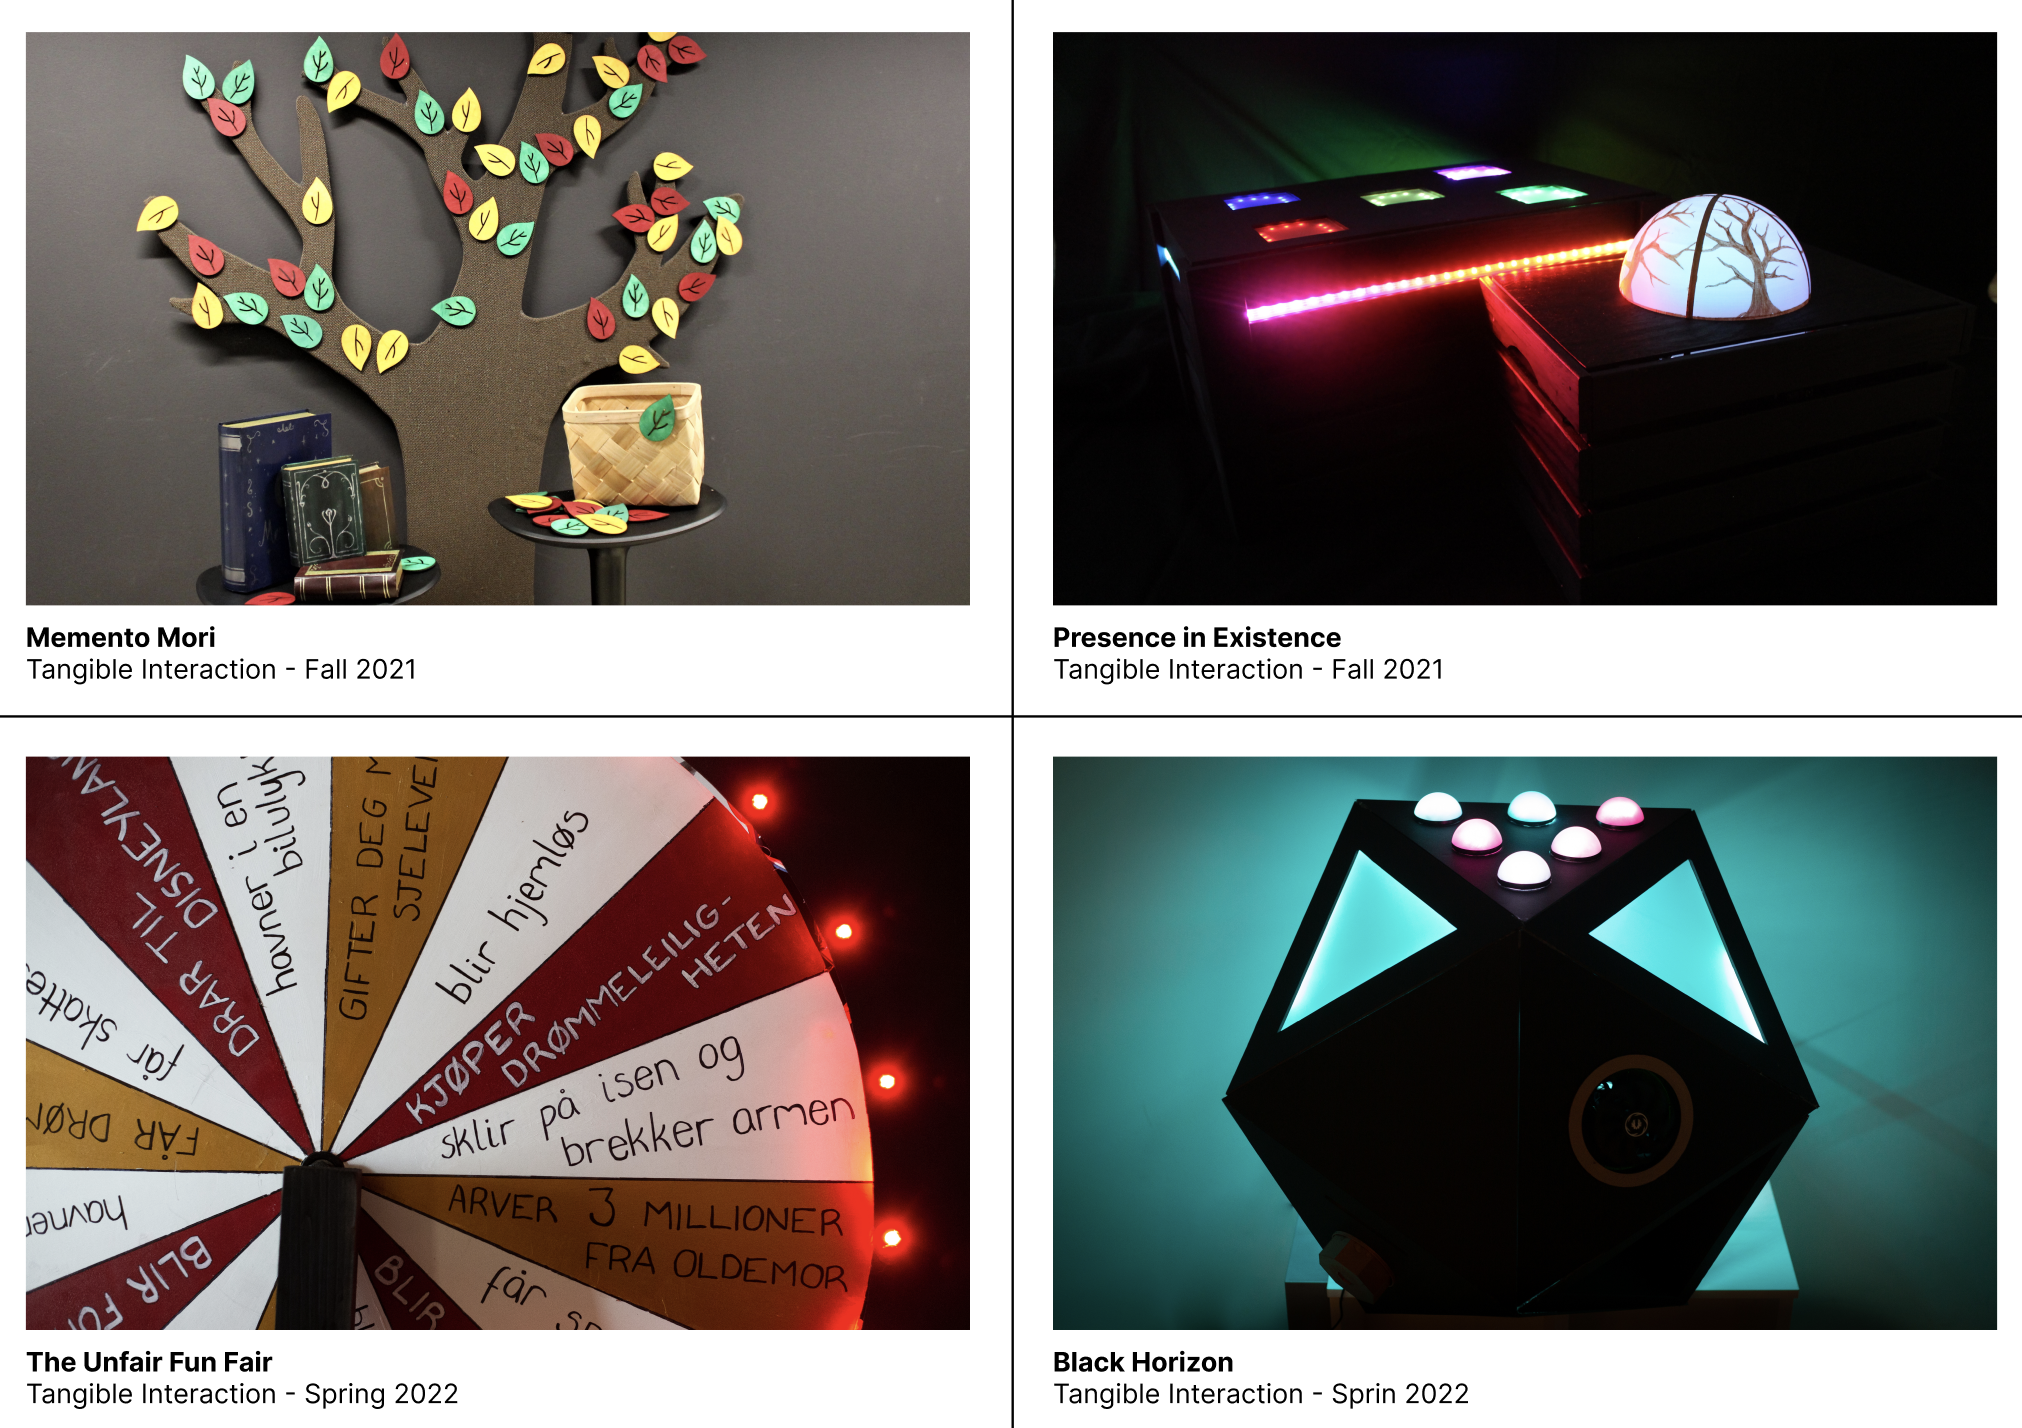
\includegraphics[width=13cm]{pictures/dataset/tangible.png}
\centering 
\end{figure}

\begin{figure}[H]
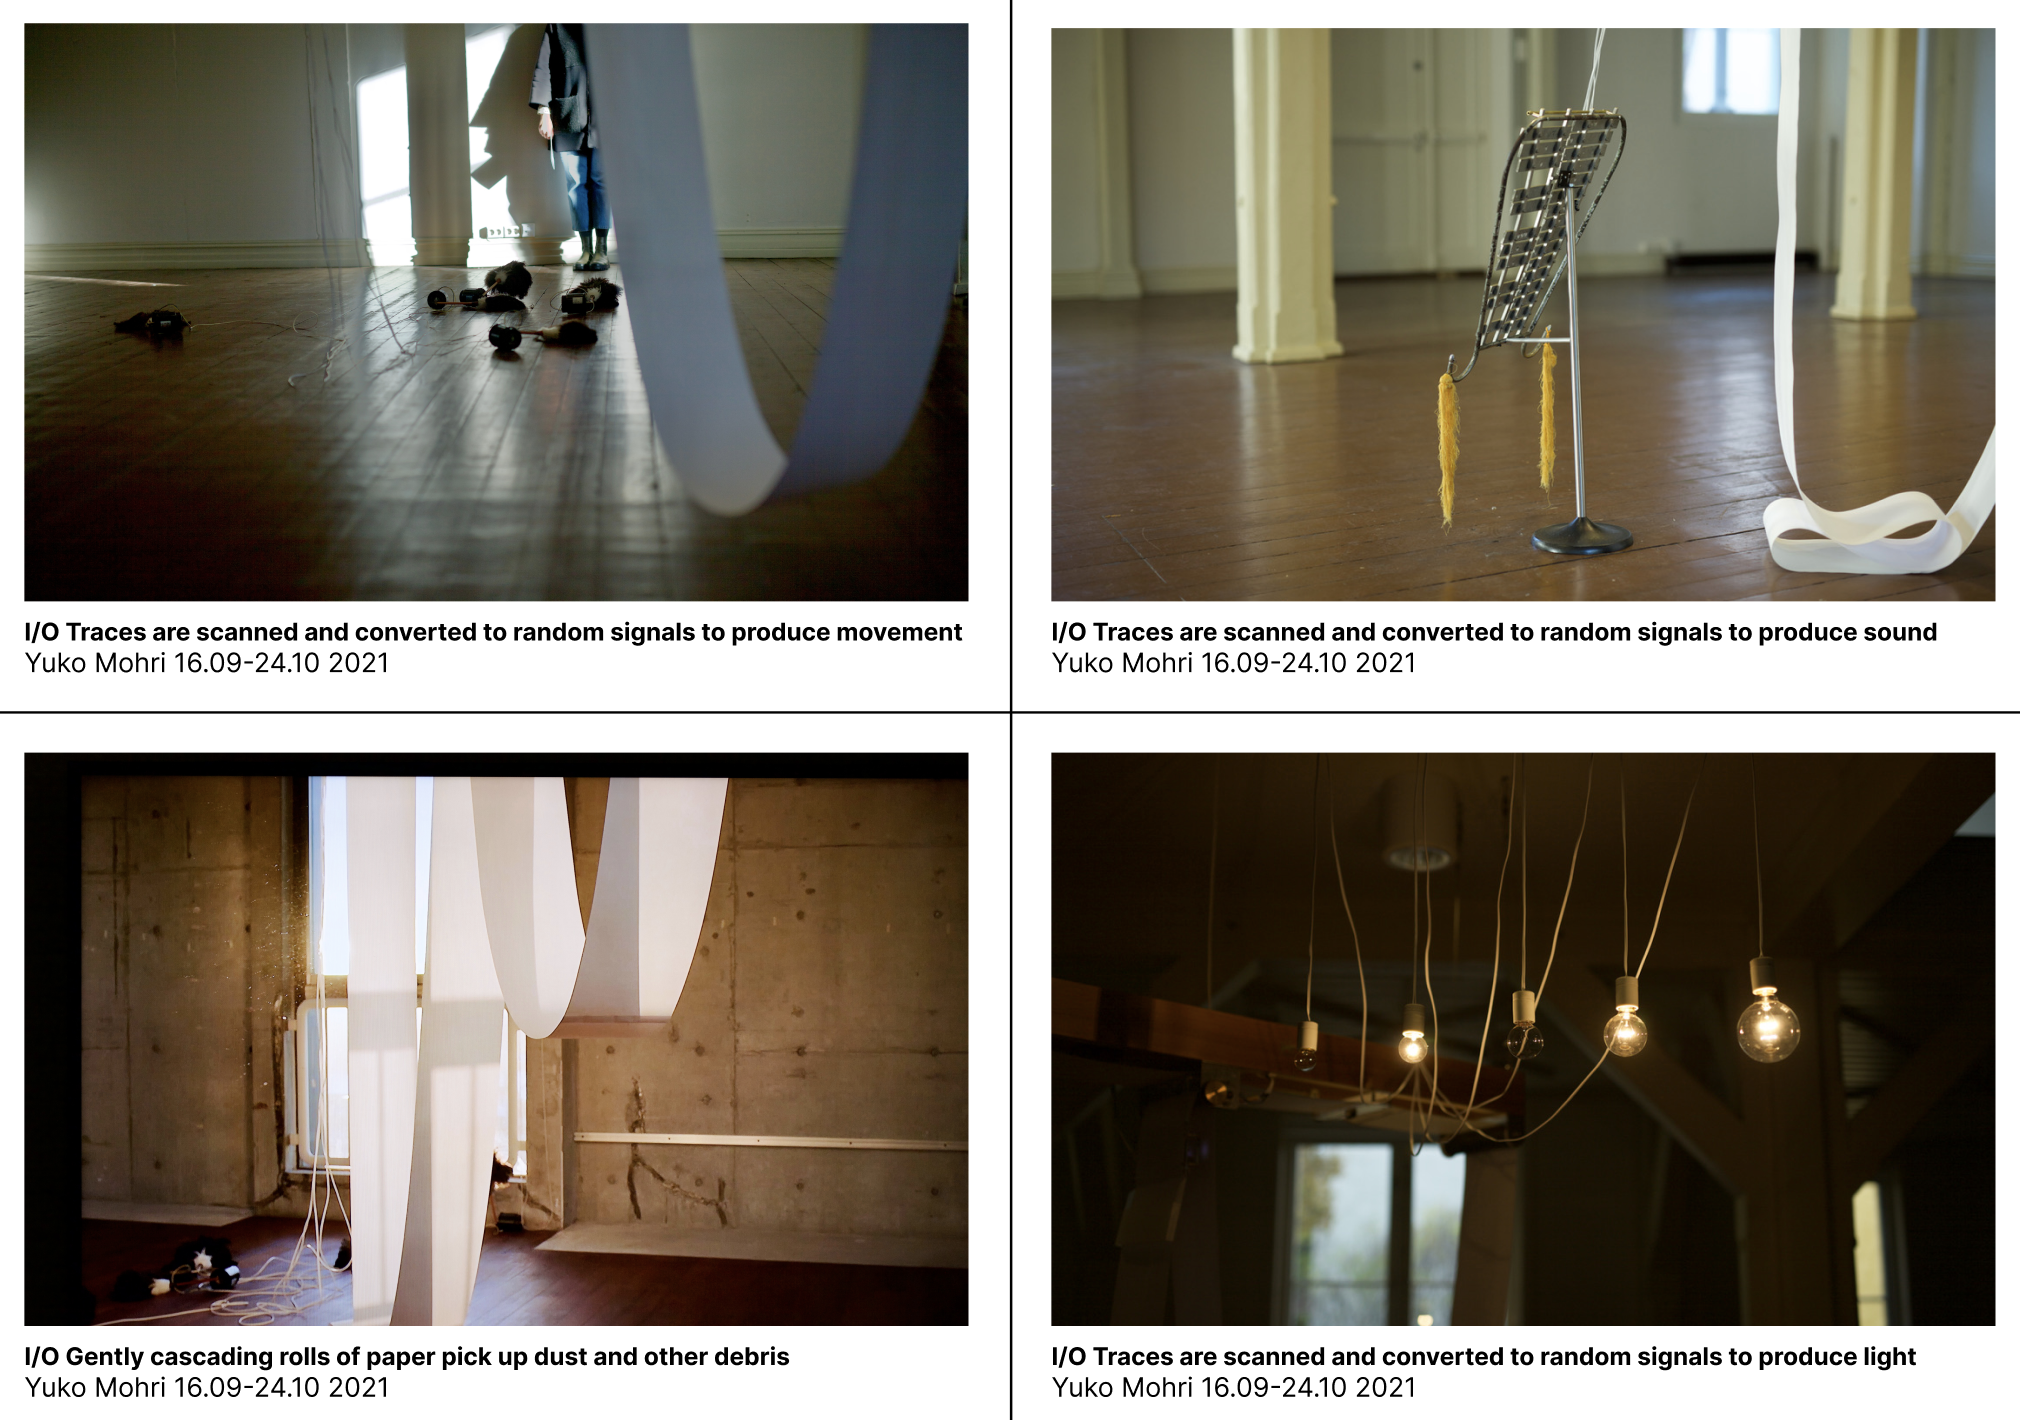
\includegraphics[width=13cm]{pictures/dataset/yuko_mohri.png}
\centering 
\end{figure}

\section{Consent forms}

\section{Analysis}
Here comes the datasets used throughout the analysis process, as written in chapter. To do:

\begin{itemize}
    \item correspondance base table
    \item radar chart x3
\end{itemize}


\subsection{Hybrid place dataset}
\begin{figure}[H]
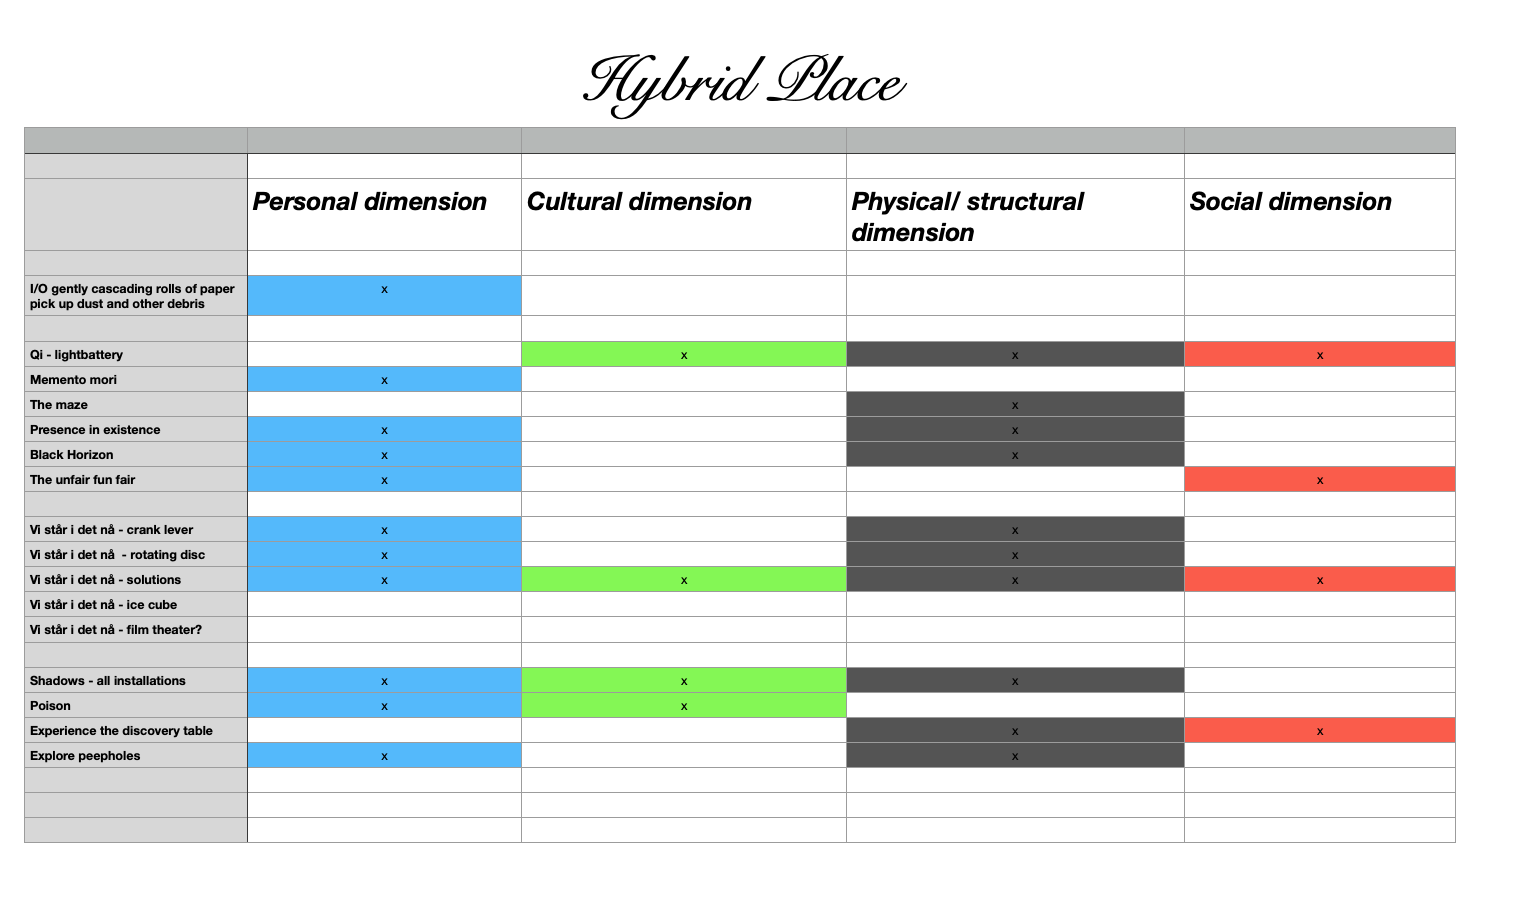
\includegraphics[width=13cm]{pictures/appendix/table_hybridplace.png}
\centering 
\end{figure}

\subsection{Place as a dialogue dataset}
\begin{figure}[H]
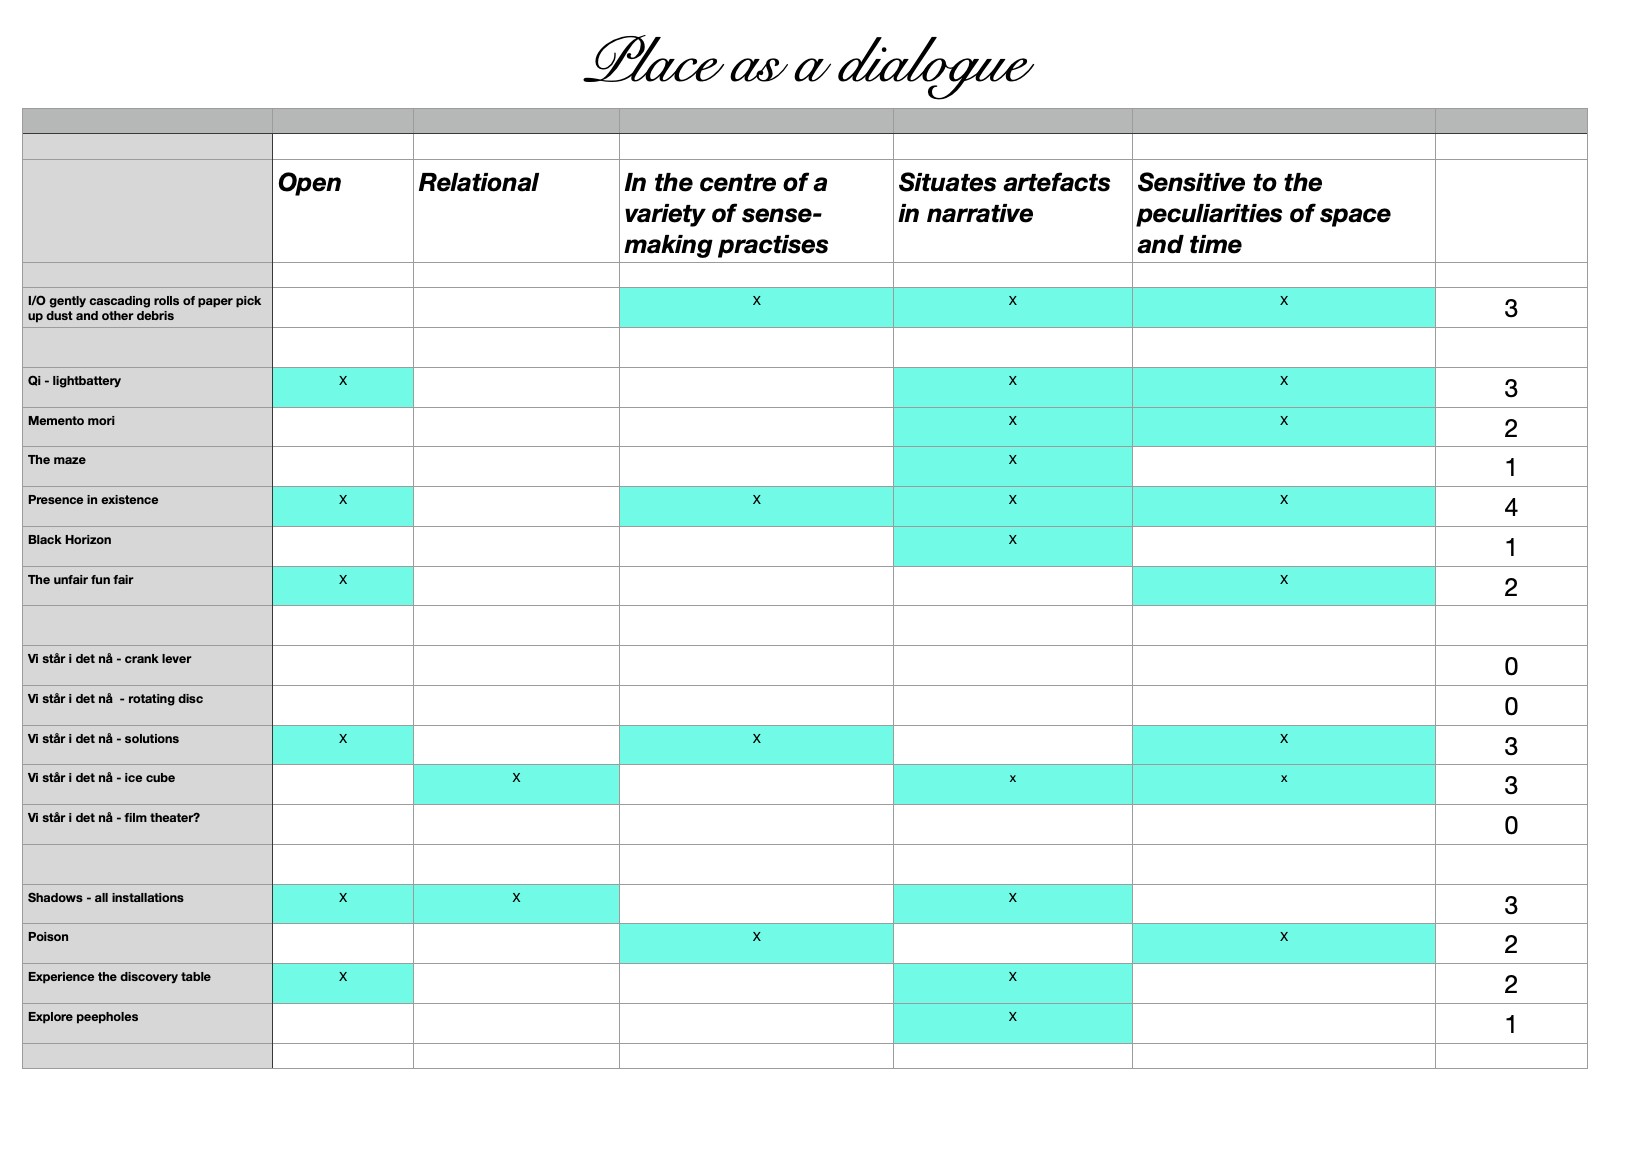
\includegraphics[width=13cm]{pictures/appendix/table_placedialogue.png}
\centering 
\end{figure}

\subsection{Sense-making strategies dataset}
\begin{figure}[H]
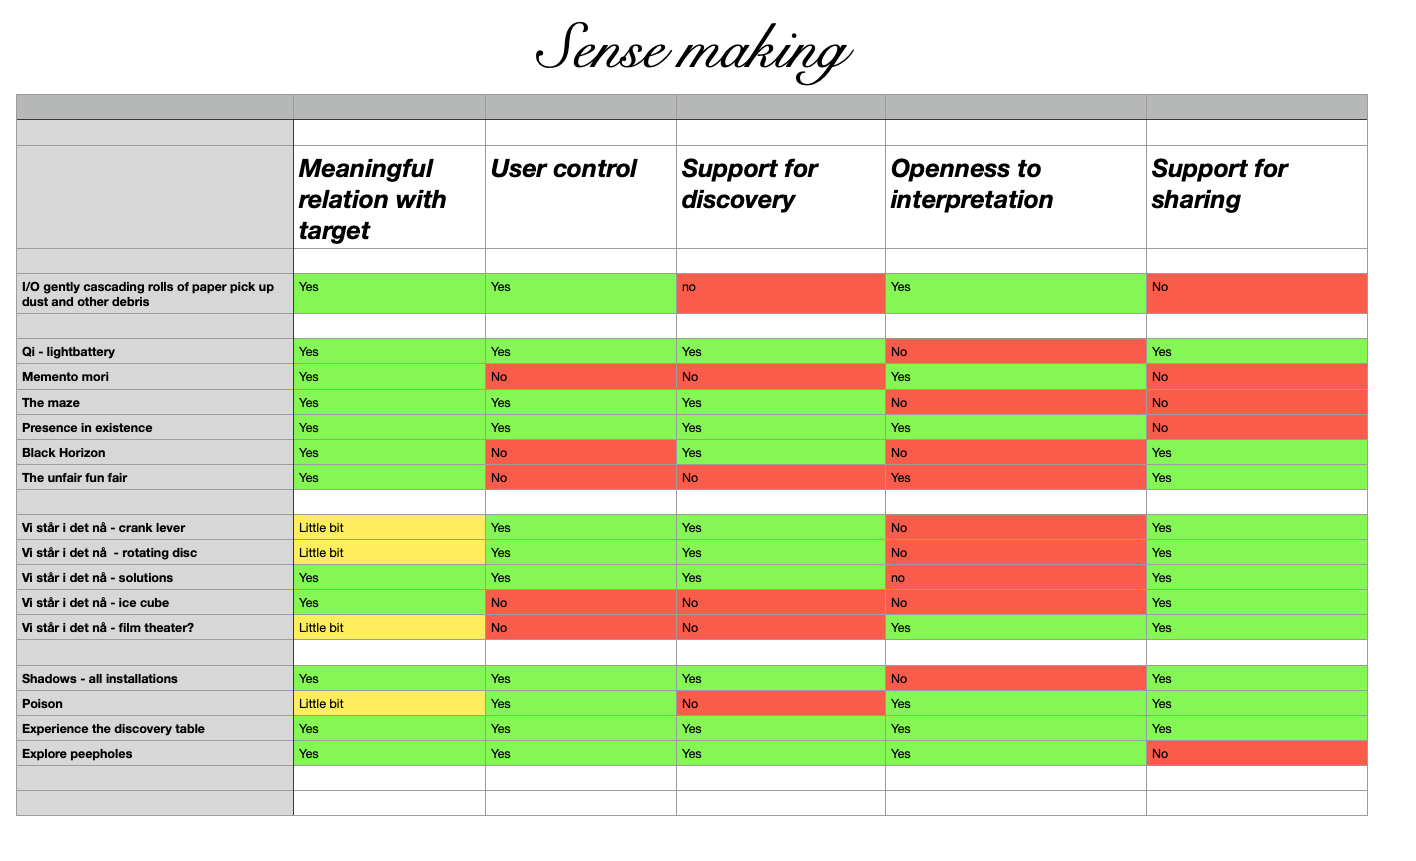
\includegraphics[width=13cm]{pictures/appendix/table_sensemaking.png}
\centering 
\end{figure}


